\documentclass[journal,12pt,twocolumn]{IEEEtran}

\usepackage{setspace}
\usepackage{gensymb}
\singlespacing
\usepackage[cmex10]{amsmath}

\usepackage{amsthm}

\usepackage{mathrsfs}
\usepackage{txfonts}
\usepackage{stfloats}
\usepackage{bm}
\usepackage{cite}
\usepackage{cases}
\usepackage{subfig}

\usepackage{longtable}
\usepackage{multirow}

\usepackage{enumitem}
\usepackage{mathtools}
\usepackage{steinmetz}
\usepackage{tikz}
\usepackage{circuitikz}
\usepackage{verbatim}
\usepackage{tfrupee}
\usepackage[breaklinks=true]{hyperref}
\usepackage{graphicx}
\usepackage{tkz-euclide}

\usetikzlibrary{calc,math}
\usepackage{listings}
    \usepackage{color}                                            %%
    \usepackage{array}                                            %%
    \usepackage{longtable}                                        %%
    \usepackage{calc}                                             %%
    \usepackage{multirow}                                         %%
    \usepackage{hhline}                                           %%
    \usepackage{ifthen}                                           %%
    \usepackage{lscape}     
\usepackage{multicol}
\usepackage{chngcntr}

\DeclareMathOperator*{\Res}{Res}

\renewcommand\thesection{\arabic{section}}
\renewcommand\thesubsection{\thesection.\arabic{subsection}}
\renewcommand\thesubsubsection{\thesubsection.\arabic{subsubsection}}

\renewcommand\thesectiondis{\arabic{section}}
\renewcommand\thesubsectiondis{\thesectiondis.\arabic{subsection}}
\renewcommand\thesubsubsectiondis{\thesubsectiondis.\arabic{subsubsection}}


\hyphenation{op-tical net-works semi-conduc-tor}
\def\inputGnumericTable{}                                 %%

\lstset{
%language=C,
frame=single, 
breaklines=true,
columns=fullflexible
}
\begin{document}

\newcommand{\BEQA}{\begin{eqnarray}}
\newcommand{\EEQA}{\end{eqnarray}}
\newcommand{\define}{\stackrel{\triangle}{=}}
\bibliographystyle{IEEEtran}
\raggedbottom
\setlength{\parindent}{0pt}
\providecommand{\mbf}{\mathbf}
\providecommand{\pr}[1]{\ensuremath{\Pr\left(#1\right)}}
\providecommand{\qfunc}[1]{\ensuremath{Q\left(#1\right)}}
\providecommand{\sbrak}[1]{\ensuremath{{}\left[#1\right]}}
\providecommand{\lsbrak}[1]{\ensuremath{{}\left[#1\right.}}
\providecommand{\rsbrak}[1]{\ensuremath{{}\left.#1\right]}}
\providecommand{\brak}[1]{\ensuremath{\left(#1\right)}}
\providecommand{\lbrak}[1]{\ensuremath{\left(#1\right.}}
\providecommand{\rbrak}[1]{\ensuremath{\left.#1\right)}}
\providecommand{\cbrak}[1]{\ensuremath{\left\{#1\right\}}}
\providecommand{\lcbrak}[1]{\ensuremath{\left\{#1\right.}}
\providecommand{\rcbrak}[1]{\ensuremath{\left.#1\right\}}}
\theoremstyle{remark}
\newtheorem{rem}{Remark}
\newcommand{\sgn}{\mathop{\mathrm{sgn}}}
\providecommand{\abs}[1]{\vert#1\vert}
\providecommand{\res}[1]{\Res\displaylimits_{#1}} 
\providecommand{\norm}[1]{\lVert#1\rVert}
%\providecommand{\norm}[1]{\lVert#1\rVert}
\providecommand{\mtx}[1]{\mathbf{#1}}
\providecommand{\mean}[1]{E[ #1 ]}
\providecommand{\fourier}{\overset{\mathcal{F}}{ \rightleftharpoons}}
%\providecommand{\hilbert}{\overset{\mathcal{H}}{ \rightleftharpoons}}
\providecommand{\system}{\overset{\mathcal{H}}{ \longleftrightarrow}}
	%\newcommand{\solution}[2]{\textbf{Solution:}{#1}}
\newcommand{\solution}{\noindent \textbf{Solution: }}
\newcommand{\cosec}{\,\text{cosec}\,}
\providecommand{\dec}[2]{\ensuremath{\overset{#1}{\underset{#2}{\gtrless}}}}
\newcommand{\myvec}[1]{\ensuremath{\begin{pmatrix}#1\end{pmatrix}}}
\newcommand{\mydet}[1]{\ensuremath{\begin{vmatrix}#1\end{vmatrix}}}
\numberwithin{equation}{subsection}
\makeatletter
\@addtoreset{figure}{problem}
\makeatother
\let\StandardTheFigure\thefigure
\let\vec\mathbf
\renewcommand{\thefigure}{\theproblem}
\def\putbox#1#2#3{\makebox[0in][l]{\makebox[#1][l]{}\raisebox{\baselineskip}[0in][0in]{\raisebox{#2}[0in][0in]{#3}}}}
     \def\rightbox#1{\makebox[0in][r]{#1}}
     \def\centbox#1{\makebox[0in]{#1}}
     \def\topbox#1{\raisebox{-\baselineskip}[0in][0in]{#1}}
     \def\midbox#1{\raisebox{-0.5\baselineskip}[0in][0in]{#1}}
\vspace{3cm}
\title{ EE3900 : Gate Assignment-1}
\author{Nelakuditi Rahul Naga - AI20BTECH11029}
\maketitle
\newpage
\bigskip
\renewcommand{\thefigure}{\theenumi}
\renewcommand{\thetable}{\theenumi}

Download all python codes from 
\begin{lstlisting}
https://github.com/Rahul27n/EE3900/blob/main/Gate_Assignment_1/Gate_Assignment_1.py
\end{lstlisting}
%
and latex-tikz codes from 
%
\begin{lstlisting}
https://github.com/Rahul27n/EE3900/blob/main/Gate_Assignment_1/Gate_Assignment_1.tex
\end{lstlisting}

\vspace{0.5cm}
\section{QUESTION: Q.33 EC-GATE-2016}

The Discrete Fourier Transform (DFT) of the 4 point sequence $ x[n] =\{3, 2, 3, 4\}$ is given by $ X[k] =\{12, 2j, 0, -2j\}$. If $X_{1}[k]$ is the DFT of the 12 point sequence $ x_{1}[n] =\{3, 0, 0, 2, 0, 0, 3, 0, 0, 4, 0, 0\}$ , the value of $\big|{\frac{X_{1}[8]}{X_{1}[11]}}\big|$ is :
\section{SOLUTION}
\vspace{0.5cm}
The 4-point DFT matrix is given by:
\begin{align}
\vec{W_{4}} &=\myvec{
 1  & 1 & 1 & 1 \\
 1 & \omega^1  &\omega^2  &\omega^3  \\
 1 & \omega^2  &\omega^4  &\omega^6  \\
 1 & \omega^3  &\omega^6  &\omega^9  \\}\\
&=\myvec{
1 &  1 &  1 &  1\\
1 &  -j & -1 & j\\
1 & -1 &  1 & -1\\
1 & j & -1 & -j}
\end{align}
where $\omega = e^{\dfrac{-2 \pi j}{4}} = -j.$
Now from the given information we can write:
\begin{align}
\vec{X} = \vec{W_{4}}\vec{x} \label{eq:1}
\end{align}
where
\begin{align}
\vec{x} &=\myvec{3 \\ 2 \\ 3 \\ 4 }
\end{align}
and 
\begin{align}
\vec{X}&=\myvec{12 \\ 2j \\ 0 \\ -2j}  
\end{align}
Now we need to find $\vec{X_{1}}$ satisfying the relation :
\begin{align}
\vec{X_{1}} = \vec{W_{12}}\vec{x_{1}} \label{eq:2}  
\end{align}
where
\begin{align}
\vec{x_{1}} &=\myvec{3 \\ 0 \\ 0 \\ 2 \\ 0 \\ 0 \\ 3 \\ 0 \\ 0 \\ 4 \\ 0 \\ 0}
\end{align}
and $\vec{W_{12}}$ is the 12-point DFT matrix which is given by:
\setcounter{MaxMatrixCols}{20}
\setlength\arraycolsep{2pt}
\begin{align}
\myvec{\textcolor{red}{1} & 1 & 1 & \textcolor{red}{1} & 1 & 1 & \textcolor{red}{1} & 1 & 1 & \textcolor{red}{1} & 1 & 1\\
\textcolor{red}{1} & \Omega & \Omega^2 & \textcolor{red}{-j} & -j\Omega & -j\Omega^2 & \textcolor{red}{-1} & -\Omega  & -\Omega^2 & \textcolor{red}{j} & j\Omega & j\Omega^2\\
\textcolor{red}{1} & \Omega^2 & -j\Omega & \textcolor{red}{-1} & -\Omega^2 & j\Omega & \textcolor{red}{1} & \Omega^2 & -j\Omega & \textcolor{red}{-1} & -\Omega^2 & j\Omega\\
\textcolor{red}{1} & -j & -1 & \textcolor{red}{j} & 1 & -j & \textcolor{red}{-1} & j & 1 & \textcolor{red}{-j} & -1 & j\\
\textcolor{red}{1} & -j\Omega & -\Omega^2 & \textcolor{red}{1} & -j\Omega & -\Omega^2 & \textcolor{red}{1} & -j\Omega & -\Omega^2 & \textcolor{red}{1} & -j\Omega & -\Omega^2\\
\textcolor{red}{1} & -j\Omega^2 & j\Omega & \textcolor{red}{-j} & -\Omega^2 & \Omega & \textcolor{red}{-1} & j\Omega^2 & -j\Omega & \textcolor{red}{j} & \Omega^2 & -\Omega\\
\textcolor{red}{1} & -1 & 1 & \textcolor{red}{-1} & 1 & -1 & \textcolor{red}{1} & -1 & 1 & \textcolor{red}{-1} & 1 & -1\\
\textcolor{red}{1} & -\Omega & \Omega^2 & \textcolor{red}{j} & -j\Omega & j\Omega^2 & \textcolor{red}{-1} & \Omega & -\Omega^2 & \textcolor{red}{-j} & j\Omega & -j\Omega^2\\
\textcolor{red}{1} & -\Omega^2 & -j\Omega & \textcolor{red}{1} & -\Omega^2 & -j\Omega & \textcolor{red}{1} & -\Omega^2 & -j\Omega & \textcolor{red}{1} & -\Omega^2 & -j\Omega\\
\textcolor{red}{1} & j & -1 & \textcolor{red}{-j} & 1 & j & \textcolor{red}{-1} & -j & 1 & \textcolor{red}{j} & -1 & -j\\
\textcolor{red}{1} & j\Omega & -\Omega^2 & \textcolor{red}{-1} & -j\Omega & \Omega^2 & \textcolor{red}{1} & j\Omega  & -\Omega^2 & \textcolor{red}{-1} & -j\Omega & \Omega^2\\
\textcolor{red}{1} & j\Omega^2 & j\Omega & \textcolor{red}{j} & -\Omega^2 & -\Omega & \textcolor{red}{-1} & -j\Omega^2 & -j\Omega & \textcolor{red}{-j} & \Omega^2 & \Omega}\nonumber
\end{align}
where
\begin{align}
\Omega &= e^{\dfrac{-2 \pi j}{12}}\\
&= \frac{\sqrt{3}-j}{2}
\end{align}
We can express $\vec{x_{1}}$ in terms of $\vec{x}$ as follows :
\begin{align}
\vec{x_{1}} &= \vec{A}\vec{x}
\end{align}
where
\begin{align}
\vec{A} &= \myvec{1 & 0 & 0 & 0 \\ 0  & 0 & 0 & 0 \\ 0  & 0 & 0 & 0\\ 0 & 1 & 0 & 0 \\ 0  & 0 & 0 & 0 \\ 0  & 0 & 0 & 0\\ 0 & 0 & 1 & 0\\ 0  & 0 & 0 & 0\\ 0  & 0 & 0 & 0\\0 & 0 & 0 & 1\\ 0  & 0 & 0 & 0\\ 0 & 0 & 0 & 0}\\
\implies \vec{A} &= \myvec{\vec{e_{1}} & \vec{e_{4}} & \vec{e_{7}} & \vec{e_{10}}}
\end{align}
where $\vec{e_{1}},\vec{e_{4}},\vec{e_{7}},\vec{e_{10}}$ represent the unit basis vectors in a subspace of $\mathbb{R}^{12}$. Now from \eqref{eq:2} have :
\begin{align}
\vec{X_{1}} = (\vec{W_{12}}\vec{A})\vec{x}
\end{align}
Only the red coloured columns in $\vec{W_{12}}$ give non-zero output when multiplied with $\vec{A}$. We can express the matrix $\vec{W_{12}}$ as a block matrix in the following way:
\begin{align}
\vec{W_{12}} = \myvec{\textcolor{red}{\vec{c_{1}}} & \vec{c_{2}} &\vec{c_{3}} &\textcolor{red}{\vec{c_{4}}} &\vec{c_{5}} &\vec{c_{6}} &\textcolor{red}{\vec{c_{7}}} &\vec{c_{8}} &\vec{c_{9}} &\textcolor{red}{\vec{c_{10}}} &\vec{c_{11}} &\vec{c_{12}}}
\end{align}
where $\vec{c_{i}}$ is the $i^{th}$ column matrix of $\vec{W_{12}}$.
Now we have:
\begin{align}
\vec{X_{1}} &= \myvec{\textcolor{red}{\vec{c_{1}}} & \vec{c_{2}} &\vec{c_{3}} &\textcolor{red}{\vec{c_{4}}} &\vec{c_{5}} &\vec{c_{6}} &\textcolor{red}{\vec{c_{7}}} &\vec{c_{8}} &\vec{c_{9}} &\textcolor{red}{\vec{c_{10}}} &\vec{c_{11}} &\vec{c_{12}}}
\vec{A}\vec{x}\nonumber\\
\implies \vec{X_{1}} &= \myvec{\textcolor{red}{\vec{c_{1}}} &\textcolor{red}{\vec{c_{4}}} &\textcolor{red}{\vec{c_{7}}} &\textcolor{red}{\vec{c_{10}}}}\vec{x}\label{eq:3}
\end{align}
We can also express $\vec{W_{4}}$ as block matrix as follows:
\begin{align}
\vec{W_{4}} = \myvec{\vec{w_{1}} &\vec{w_{2}} &\vec{w_{3}} &\vec{w_{4}}}
\end{align}
where $\vec{w_{i}}$ is the $i^{th}$ column matrix of $\vec{W_{4}}$.

We can importantly note that :
\begin{align}
\vec{c_{1}} &= \myvec{1 \\ 1 \\ 1} \otimes \vec{w_{1}}\\
\vec{c_{4}} &= \myvec{1 \\ 1 \\ 1} \otimes \vec{w_{2}}\\
\vec{c_{7}} &= \myvec{1 \\ 1 \\ 1} \otimes \vec{w_{3}}\\
\vec{c_{10}} &= \myvec{1 \\ 1 \\ 1} \otimes \vec{w_{4}}
\end{align}
where $\otimes$ represents the \textbf{Kronecker Product}.

Therefore from \eqref{eq:3} we have:
\begin{align}
\vec{X_{1}} &= \myvec{1 \\ 1 \\ 1} \otimes \myvec{\vec{w_{1}} & \vec{w_{2}} & \vec{w_{3}} & \vec{w_{4}}}\vec{x}\\
&= \myvec{1 \\ 1 \\ 1} \otimes \vec{X}\\
&= \myvec{12 \\ 2j \\ 0 \\ -2j \\ 12 \\ 2j \\ 0 \\ -2j \\ 12 \\ 2j \\ 0 \\-2j}
\end{align}
Therefore we have:
\begin{align}
\Big|{\frac{\vec{X_{1}}[8]}{\vec{X_{1}}[11]}}\Big| = \Big|{\frac{12}{-2j}}\Big| =\big|6j\big| = 6
\end{align}

\begin{figure}[!ht]
    \centering
    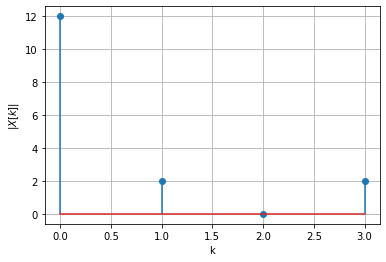
\includegraphics[width=\columnwidth] {Gate_Assignment_1_Fig_1.png}
    \caption{Magnitude of $\vec{X}[k]$ vs $k$}
    \label{Magnitude of X[k]}
\end{figure}

\begin{figure}[!ht]
    \centering
    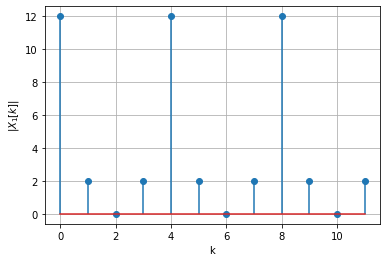
\includegraphics[width=\columnwidth] {Gate_Assignment_1_Fig_2.png}
    \caption{Magnitude of $\vec{X_{1}}[k]$ vs $k$}
    \label{Magnitude of X1[k]}
\end{figure}

\end{document}
